
\documentclass{beamer}

\usetheme{CambridgeUS}
%\usecolortheme{albatross}

\usepackage{graphicx} 
\usepackage{booktabs} 

\title[Week 2 Review]{EPSRC Vacation Scheme: Week 2 Review} 

\author{Matthew Knowles} 
\institute[UoY] 
{
Department of Mathematics \\
University of York \\ 
\medskip
\textit{mk1320@york.ac.uk} 
}
\date{$2^{nd}$ August 2021} 

\begin{document}

\begin{frame}
\titlepage 
\end{frame}



\begin{frame}
\frametitle{Goals of last week}
\begin{enumerate}
	\item Implement searching aspect of the Roux Algorithm 
	\pause
	\item Implement Quickhull
	\pause
	\item Run performance test comparrison on all 3 algorithms
	\pause
	\item Xu's Thesis
\end{enumerate}
\end{frame}

\begin{frame}
\frametitle{Task 1 Progress}
\begin{itemize}
	\item Relatively easy to fix, and gave massive improvement on performance
	\pause
	\item Let Python randomly generate functions to test on.  
	\pause
	\item This time, they are perfect
\end{itemize}
\end{frame}

\begin{frame}
\frametitle{First test}
	\begin{figure}
		\center
		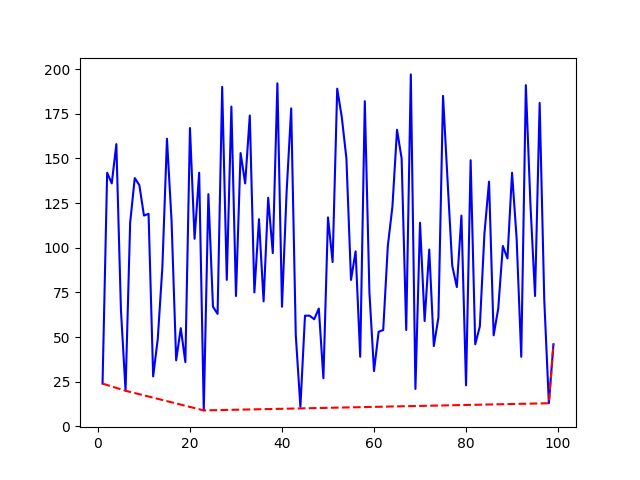
\includegraphics[scale=0.6]{../Figures/Figure_10.png}
	\end{figure}
\end{frame}

\begin{frame}
\frametitle{Second test}
	\begin{figure}
		\center
		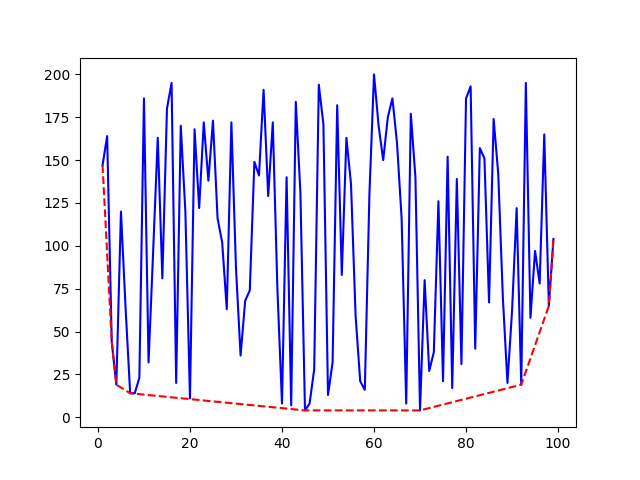
\includegraphics[scale=0.6]{../Figures/Figure_11.png}
	\end{figure}
\end{frame}

\begin{frame}
\frametitle{Comparrison with Monotone-Chain}
\begin{itemize}
	\item Next task was to comapre this with Monotone Chain
	\pause
	\item Can see that it is slightly slower, but both run in $\mathcal{O}(n)$ time!
	\pause
	\item A lot more variation in times, not sure why this is
\end{itemize}
\end{frame}

\begin{frame}
\frametitle{Roux VS Monotone-Chain}
	\begin{figure}
		\center
		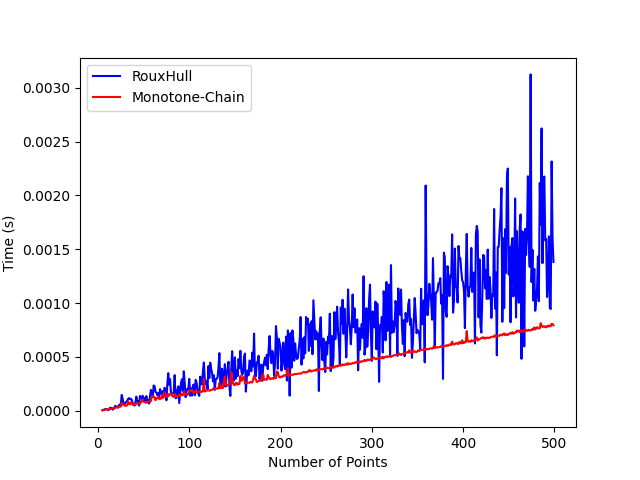
\includegraphics[scale=0.6]{../Figures/rouxVSmono.png}
	\end{figure}
\end{frame}

\begin{frame}
\frametitle{Quickhull}
\begin{itemize}
	\item This is possibly the most frustrating piece of code I have ever written
	\pause 
	\item Upside: Very quick, it runs quicker than both other algorithms
	\pause
	\item Note: My implementation isn't perfect, a few edge cases don't work properly
\end{itemize}
\end{frame}

\begin{frame}
\frametitle{Complete Comparrison}
	\begin{figure}
		\center
		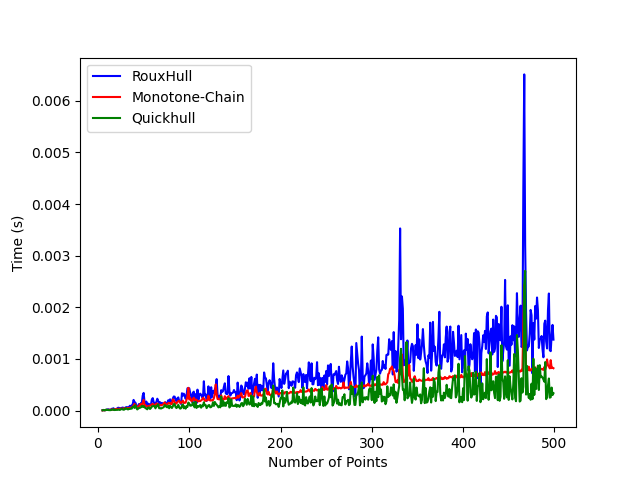
\includegraphics[scale=0.6]{../Figures/full_comparison.png}
	\end{figure}
\end{frame}

\begin{frame}
\frametitle{Xu's Thesis}
\begin{itemize}
	\item Began going through Chapter 4.1
	\pause
	\item Making good progress with understanding material
	\pause
	\item This week I would like to try implementing some of this?
\end{itemize}
\end{frame}
	

\begin{frame}
\Huge{\centerline{Any Questions?}}
\end{frame}


\end{document} 